\documentclass[toc=flat,fontsize=11pt,a4paper,titlepage,headsepline,numbers=noenddot, bibliography=totoc]{scrartcl}
%\setcounter{secnumdepth}{5}
%\setcounter{tocdepth}{5}
\usepackage[utf8]{inputenc}
\usepackage[ngerman]{babel} 
\usepackage[T1]{fontenc}
\usepackage{graphicx}
\graphicspath{{images/},{.}}
\usepackage{listings}
%\usepackage{setspace}
\usepackage[automark]{scrpage2}

\usepackage[colorinlistoftodos,prependcaption,textsize=tiny]{todonotes} % wegen ToDo

\PassOptionsToPackage{hyphens}{url}\usepackage{hyperref} % Hyperlinks

\usepackage{csquotes} 
\usepackage[backend=bibtex,bibencoding=ascii,style=numeric]{biblatex} %style=authoryear
\bibliography{biblio}

\apptocmd{\UrlBreaks}{\do\f\do\m}{}{}
\setcounter{biburllcpenalty}{9000}% Kleinbuchstaben
\setcounter{biburlucpenalty}{9000}% Großbuchstaben

\pagestyle{scrheadings}
\author{Sven Sengpiehl}
\ohead[]{\pagemark}

 \def\bf{\normalfont\bfseries}

\begin{document}

\thispagestyle{empty}

\hspace{20cm}
\vspace{-2cm}

\begin{center}
  \vspace{0.5 cm}
  \huge{\bf Virtualisierungmöglichkeit der Altersverifikation mit Hilfe des neuen Personalausweises \linebreak\linebreak 
\includegraphics[width=6 cm]{HU_Logo}} \\
  \vspace{1.5cm}
  {\large
    \bf{
      %\scshape
      Humboldt-Universit\"at zu Berlin \\
      Mathematisch-Naturwissenschaftliche Fakult\"at II \\
      Institut f\"ur Informatik\\
    }
  } 
  \vspace{1cm}
  \LARGE Studienarbeit \\
  \vspace{2cm}
  \normalsize
      Sven Sengpiehl\\
    \vspace{0.5cm}
      \today\\
\vspace{1cm}
    Betreuer:
    \vspace{0.5cm}
    Dr. Wolf Müller \\
  % \normalfont
\end{center}
\vspace {5 cm}% gegebenenfalls kleiner, falls der Titel der Arbeit sehr lang sein sollte
%{3.2 cm} bei Verwendung von scrreprt, gegebenenfalls kleiner, falls der Titel der Arbeit sehr lang sein sollte

\newpage
\thispagestyle{empty}
\LARGE
\begin{center}


\bf{ Zusammenfassung}
\end{center}
\normalsize
\noindent


\newpage
\thispagestyle{empty}
\tableofcontents

\newpage

\section{Motivation}
Mit der Einführung des neuen Personalausweises (\textit{nPA}) zum 1. November 2010 stellt dieser einen elektronischen Identitätsnachweis zur Verfügung.
Gegenüber dritten Parteien ist man in der Lage sich online zu authentisieren. Dies erspart - z.B. bei Behördengängen oder Eröffnung eines Kontos - die Sichtprüfungen.
Für diesen Vorgang ist das Auslesen personenbezogener Daten - in Form von Datengruppen (\textit{DG}) - aus dem Ausweis notwendig.\\ 
Zusätzlich bietet der nPA weitere Funktionen an. Im Zuge dieser Arbeit wird die Altersverifikation betrachtet. Diese wird z.B. auf nicht jugendfreien Seiten oder beim 
Einkaufen benötigt. 

Im Folgenden wird untersucht, ob die Funktion der Altersverifikation des nPA als Dienst zur Verfügung gestellt werden kann. Der Ausweis arbeitet dabei im Verborgenem. 
Der Nutzer des Dienstes hat keinen physischen Zugriff auf die Karte; lediglich der Betreiber des Dienstes hat die Hoheit über den Ausweis. Die einzelnen Datengruppen 
können vom Nutzer nicht ausgelesen werden; vom Ausweis werden keine persönlichen Daten des Ausweisinhabers gesendet. Die Bereitstellung des nPA nach außen 
kann anonym stattfinden.

\section{Datenaustausch zwischen den beteiligten Parteien}
\todo[inline]{Skizze, Begriffe\\
Remoteterminal, lokales Terminal(Lesegerät), Dienstanbieter(eID-Dienst), eID-Client\\
Bitte beachten Sie, dass Sie für diesen Vorgang eine Internetverbindung benötigen. Dies hat folgenden Hintergrund: Für jedes Auslesen der Daten aus dem 
Personalausweis oder dem elektronischen Aufenthaltstitel muss gesetzlich der Zweck des Auslesevorgangs angegeben werden. Dieser Zweck wird Ihnen auf 
einem speziellen Zertifikat angezeigt (Berechtigungszertifikat). Diese Zertifikate werden individuell durch die Vergabestelle für Berechtigungszertifikate beim
 Bundesverwaltungsamt genehmigt. Damit Sie also jederzeit genau wissen, wer zu welchem Zweck einen Auslesevorgang startet, wird eine Internetverbindung 
 zu einem vertrauenswürdigen Authentisierungsserver aufgebaut. Die Berechtigungszertifikate dienen Ihrem Schutz!
}

\section{Schutzmechanismen}

Der nPA ist als kontaktlose Chipkarte gemäß ISO 14443 \cite{ISO14443} implementiert. Sobald sich der nPA in Reichweite des Lesegerätes befindet, kann - durch das 
Lesegerät inititert - die Übertragung der Daten beginnen. Die Luftschnittstelle stellt per se kein abhörsicheres  Medium dar. Daher sollten die ausgetauschten Daten 
bei der Übertragung gegen unbefugtes Mitlesen/Ändern (Authentizität/Integrität) geschützt werden; dies gewährleistet ein secure messaging-Kanal (\textit{SM}) zwischen 
Lesegerät und nPA. 

Die Daten auf dem nPA sind im dortigen Dateisystem abgelegt; können vom Dienstanbieter aber nicht direkt selektiert und ausgelesen werden. Der Zugriff auf 
die Daten und Funktionen des nPA  wird durch die \textit{General Authentication Procedure} (\textit{GA}) \cite{TR3110} kontrolliert. Die GA besteht aus den vier Schritten:
\begin{itemize}
	\item Password Authenticated Connection Establishment (\textit{PACE}) \cite{TR3110}
	\item Terminal Authentication (\textit{TA})
	\item Passive Authentication 
	\item Chip Authentication (\textit{CA}) 
\end{itemize}
Die letzten drei Schritte werden als \textit{EAC} (Extended Access Control) bezeichnet.

%ToDo:
Das Berechtigungszertifikat ist nicht nur für entfernte Dienstanbieter - auch die Lesegeräte sind mit einem solchem Zertifikat ausgestattet. Somit sind dem Lesegerät nur bestimmte Rechte zugewiesen; hierbei denke ich insbesondere an IS-Terminals, an denen bestimmte Daten auch ohne eID-Pin -nur mit CAN ausgelesen werden dürfen.

In einem für das Remoteterminal(Dienstanbieter) ausgestelltem \textit{Berechtigungszertifikat} sind dessen Zugriffsrechte hinterlegt. Bei der Abfrage von Daten durch 
das Remoteterminal werden die angestrebten Rechte in einem \textit{Card Holder Authorization Template} (CHAT) übergeben und dem Anwender vor der Ausführung 
von PACE präsentiert. Er hat die Möglichkeit diese Rechte einzuschränken. Das PACE-Protokoll leitet anschließend aus einem schwachen Geheimnis - der eID-PIN oder 
der CAN - einen starken Sitzungsschlüssel für den SM-Kanal zwischen Lesegerät und dem Ausweis ab. Nach Aufbau des SM-Kanals werden die drei Schritte der EAC in 
diesem sicheren Kanal übertragen. Der Chat und somit die geforderten Zugriffsrechte sind an die SM-Sitzung gebunden und können während derer nicht geändert werden.\\
Während der TA werden die Zugriffsrechte durch bitweise Verundung  der Chats der kompletten im Chip gespeicherten Zertifikatskette bestimmt. Dem Remoteterminal
mit seinem Berechtigungszertifikat können somit nicht mehr Rechte gegeben werden, als die in der PKI übergeordneten Instanzen erlauben. Sollte ein Zertifikat abgelaufen 
sein, kann es nachgeladen werden.\\
Das Remoteterminal kann im Gegenzug durch die CA die Gültigkeit des nPA prüfen.
Nach Abschluss der EAC ist die Authentizität der beiden Kommunikationspartner sichergestellt. Zugleich wurde ein zweiter SM-Kanal zwischen dem Remoteterminal und dem 
Chip aufgebaut. Der eID-Dienst darf die im Chat angefragten Daten auslesen bzw. Ausweisfunktionen aufrufen. 
Bei der Altersverifikation wird ein zu prüfendes Testdatum an den nPA mit übergeben, welches vom nPA mit dem hinterlegten realen Geburtsdatum 
verglichen wird. Es wird lediglich das Ergebnis des Datumsvergleiches zurückgemeldet. Somit kann das personenbezogene Geburtstdatum nicht ausgelesen werden.

\subsection{Umzusetzende Schutzziele im Rahmen dieser Arbeit}
\todo[inline]{wo genau}
Trotz den bereits implementierten Absicherungen des nPA ist dieser nicht gänzlich geschützt. Für den Inhaber des nPA darf dieser niemals unbrauchbar 
werden. Um dies zu verhindern muss ein manueller Aufbau eines PACE-Kanals untersagt werden. Ansonsten besteht die Möglichkeit mit der dreimaligen 
Fehleingabe der eID-PIN den Ausweis zu sperren.
Demzufolge muss ein zustandsbasierter Kommando(\textit+APDU)-Filter implementiert werden.

Desweiteren dürfen aus dem Ausweis nicht alle zur Verfügung stehenden Daten, trotz Berechtigung des eID-Dienstes gemäß Berechtigungszertifikat, 
ausgelesen werden. Die Anonymität des Ausweisinhabers wäre damit verletzt.  

\section{Umsetzung}

\begin{figure}[!htb]
\centering
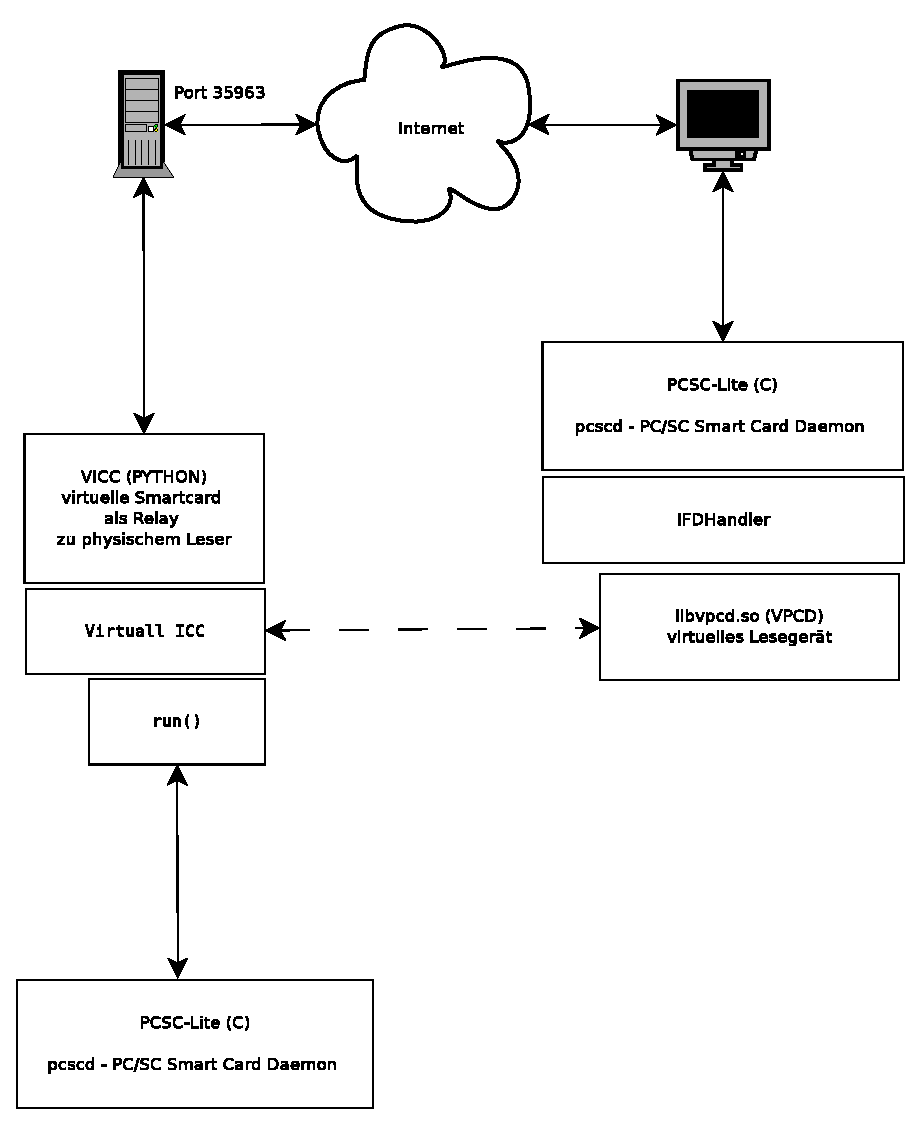
\includegraphics[scale=.75]{Kommunikationswege}
\caption{Anwendungsfall}
\label{ov}
\end{figure}

\subsection{Vorüberlegungen}

Die Benutzung eines Online-Dienstes setzt einen lokalen eID-Client voraus, der als Mittelsmann zwischen Dienst und Karte fungiert.
Im Verlauf einer Abfrage von Daten ist die wichtigste Aufgabe des eID-Clients ist die Anzeige der angeforderten Rechte aktuell benutzten Dienstes 
und dessen Berechtigungszertifikat.

Zusätzlich muss der eID-Client den Aufbau des weiter oben beschriebenen PACE-Protokolls initiieren. Dazu tauscht er mit dem Kartenlesegerät
s.g. Pseudo-APDUs (\textit{P-APDU}) aus. Diese sind in BSI TR-03119 spezifiziert. Die meisten bisher imlementierten eID-Client senden hingegen 
\verb+SCard-Kommandos+ an das Lesegrät. Der Gerätetreiber antwortet auf die P-APDU bzw. das SCard-Kommando.  

Im ersten Schritt fragt der eID-Client die Eigenschaften des Lesegerätes an. Dabei verhalten sich die Lesegeräte unterschiedlich.
Der Komfortleser führt PACE mit der Karte durch, wo hingegen beim Basisleser PACE zwischen eID-Client und
Karte mittels APDUs durchgeführt wird. Somit fällt auch die Antwort des Gerätetreibers dementsprechend aus.

Für unseren Anwendungsfall muss dem eID-Client mitgeteilt werden, dass das Lesegerät über ein PIN-Pad aber kein Display verfügt. Somit sendet der
eID-Client später das Kommando zur Ausführung von PACE mit den entsprechend in BSI TR-03119 spezifizierten Parametern.

Würde der eID-Client PACE mit der Karte selbst durchführen, könnte der Anwender die eID-PIN dreimal falsch eingeben. Die eID-Funktion des nPA
wäre gesperrt.

Im folgenden ermittelt der eID-Client anhand von APDUs, ob sich ein nPA in Reichweite des Lesegerätes befindet.
Dazu wird geprüft, ob in der Datei EF.Dir (Liste der Kartenapplikationen ) ein Eintrag \texttt{0xE80704007F00070302} vorhanden ist.

Der Clientrechner verfügt über keinen Kartenleser. Über die Implementierung einer virtuellen Smartcard von  F. Morgner und D. Oepen wird dem Client 
ein virtueller Kartenleser zur Verfügung gestellt. Der lokal laufende eID-Client verbindet sich über die pcsclite-Bibliothek mit diesem Lesegerät.
Diese virtuelle Lesegerät leitet alle eingehenden APDUs per TCP über das Netzwerk an den auf einem Host laufenden \verb+Relay+ weiter.\\ 
Die oben angeführten zusätzlichen Schutzmechanismen sind auf dem Hostrechner in diesem Relay zu implementieren. Eine Manipulation von außen ist
somit weitestgehend ausgeschlossen.

\subsection{Client}

Der von F. Morgner und D. Oepen implementierte \verb+VPCD+ der \verb+VIRTUALSMARTCARD+ muss angepasst werden.
Der eID-Client versucht über den Treiber, mit dem Aufruf des SCard-Kommandos \verb+GET_FEATURE_REQUEST+ oder der P-APDU \verb+FF9A0401+, 
die Eigenschaften des Lesegerätes zur ermitteln. Die Originalimplementierung unterstützt keine Scardcontrol-Kommandos.

Mit der Erweiterung der Standard-Implementierung - Methode \verb+ifd-vpcd.c->IFDHControl+ - werden nicht mehr alle  SCardcontrol-Kommandos verworfen.
Die folgenden drei Kommandos werden clientseitig berücksichtigt. Sie werden nicht an den Host-Rechner weitergeleitet, da der dort laufende
 VPCD mit diesen Kommandos nichts anfangen kann.

 \begin{tabular}{|l|c|c|}
 \hline
  Scardcontrol & zusätzliche Funktion & Antwort\\
  \hline
    \verb+GET_FEATURE_REQUEST+ & - & \verb+FEATURE_EXECUTE_PACE+\\
    \verb+FEATURE_EXECUTE_PACE+ & \verb+GetReaderPACECapabilities+ & \verb+PACE+ \\
    \verb+FEATURE_EXECUTE_PACE+ & \verb+establishPACEchannel+ & Ausgabe siehe BSI TR-03119 Appendix D.3 \\
    \hline
 \end{tabular} 

\textbf{GET\_FEATURE\_REQUEST}: im Datenteil der Antwort wird \verb+FEATURE_EXECUTE_PACE+ zurückgegeben. Somit versucht der
eID-Client nicht selbst den PACE-Kanal durch APDUs aufzubauen.
 
\textbf{FEATURE\_EXECUTE\_PACE} wird mit der Funktion \verb+GetReaderPACECapabilities+ aufgerufen. Dem eID-Client wird das 
PACE feature \verb+0x40+ gemeldet.
 
\textbf{FEATURE\_EXECUTE\_PACE} wird mit der Funktion \verb+establishPACEchannel+ und den notwendigen Eingabedaten für diese Funktion 
- BSI TR-03119 Appendix D.3 - aufgerufen. Bei Empfang des Kommandos werden die Daten extrahiert, an die Pseudo-APDU \texttt{FF9A0402} gehangen und 
an den entfernten Host gesendet.  

\subsection{Host}

Die Implementierung für den Host ist ein \verb+VPCD+-Relay. Dieser verbindet sich mit dem entfernten Client-VPCD und dem lokalen Kartenleser. 
Alle ankommenden APDUs werden untersucht. Falls das Kommando zulässig ist, wird die APDU mit der Funktion  \verb+sc_transmit_apdu()+
an die Karte im Kartenleser weitergeleitet.\\
Eine Ausnahme stellt die Pseudo-APDU \texttt{FF9A0402} dar. Beim Eingang wird der CHAT nach zulässigen Berechtigungen untersucht. Diese können 
beim Programmstart als Bit-Maske mitgegeben werden. Sofern die angeforderten Berechtigungen zulässig sind, wird aus der \verb+libnpa+ die 
Funktion \verb+perform_pace()+ aufgerufen. Die notwendige PIN oder CAN wird beim Programmstart mitgegeben. \\
Nach erfolgreichem Aufbau des SM-Kanals - durch PACE - zwischen Karte und Kartenleser findet die Übertragung der APDUs 
für das anschließende \textit{EAC} in diesem SM-Kanal statt.\\ 
Der SM-Kanal wird in \verb+OpenSC+ als Kontext gespeichert.
Die weitere Übertragung der APDUs zwischen externer Anwendung und der Karte findet in dem durch PACE und EAC aufgebauten zweitem SM-Kanal statt. 
Daher kann der erste SM-Kanal (PACE) geschlossen werden. 

\subsubsection{APDU-Filter}

Durch dreifach wiederholt falsche eID-PIN-Eingabe wird die eID-Funktion auf dem nPA gesperrt. Dies gilt es zu verhindern.

Die Funktionen des nPA sind nur nach erfolgreichem Aufbau des PACE-Kanals nutzbar. Für diesen wird die eID-Pin verwendet.
Die Initiierung des PACE-Kanals wird durch die folgenden APDUs erkannt und nach der APDU für $General Authenticate$ abgewiesen.

Beispiele:\\
\verb+npa-tool+:\\
APDU: \texttt{0022C1A40F800A04007F00070202040202830103}\\
APDU: \texttt{10860000027C0000}\\
\verb+eID-Client+:\\
APDU: \texttt{0022C1A427800A04007F00070202040202830103}\\
		   \texttt{84010D7F4C12060904007F00070301020253050000000001}\\ 
APDU: \texttt{10860000027C0000}\\

Zusätzlich zu den APDUs müssen die Pseudo-APDUs betrachtet werden. 
$FF9A0401 - get\_PACE\_capabilities()$ darf nicht an den Leser gesendet werden. Der Leser würde, falls dieser die PACE-Funktionalität nicht nativ unterstützt, 
dies zurückmelden und der eID-Client würde anschließend das PACE-Protokoll starten. Dieses würde aber, wie weiter oben geschrieben, abgewiesen werden.\\
$FF9A0402 - establish\_PACE\_channel()$ wird angenommen, in die Input-Parameter der Funktion  \verb+libnpa->perform_pace()+ umgewandelt und 
anschließend die Funktion \verb+perform_pace()+ aufgerufen. Die von der Funktion erhalten Werte werden in eine entsprechend gemäß \cite{TR3119} Antwort 
verpackt und an den \verb+VPCD+ des Client-Rechners gesendet.

Die Filterung der APDUs ist nicht ausreichend. Der nPA stellt bereits Schutzmechanismen für die eID-Funktion zur Verfügung.
Dem Nutzer des Dienstes darf es dennoch nur möglich sein zuvor festgelegte Daten auszulesen bzw. Funktionen des nPA zu benutzen, 
auch wenn der Dienstanbieter gemäß Berechtigungszertifikat über umfassendere Berechtigungen verfügt.
Welche Rechte dem Anwender gewährt werden, können beim Programmstart als Bitstring mitgegeben werden. 
Mittels PACE teilt das Terminal dem Chip seinen Terminaltyp und seine angestrebten Rechte mit. Diese werden im Authentisierungsprozess nachgewiesen.

Die maximalen Rechte des Remoteterminals müssen eingeschränkt werden, damit keine persönlichen Daten aus dem Ausweis ausgelesen werden können.  

\section{Testszenario}

Auf dem Hostrechner sind die folgenden Dienste/Programme aktiv
\begin{itemize}
  \item Basisleser mit nPA
  \item PCSCD mit aktiviertem Basisleser und Leser für vpcd
 % \item \deleted{\verb+vicc -t relay --reader 1(Basisleser) -H Client -vvv+}
  \item \verb+./client ...+ (Relay)
\end{itemize}

Auf dem Clientrechner sind die folgenden Dienste/Programme aktiv
\begin{itemize}
  \item PCSCD mit Leser für VPCD - \verb+pcscd -dfa+
  \item kein VICC starten
  \item eID-Client - \verb+java -jar /data/OpeneCardApp-1.0.6.jar+ - erst nach dem relay auf dem Host-Rechner starten  
\end{itemize}

Beim Starten des Relay-Programmes auf dem Hostrechner wird eine TCP-Verbindung zum Client-VPCD aufgebaut, über diese anschließend die Befehle 
ausgetauscht werden.
Die APDUs vom eID-Client werden nun über den dortigen VPCD-Leser an den Relay auf dem Host-Rechner gesendet. Dieser leitet die APDUs 
nach vorangegangener Prüfung an den Basisleser weiter.

\subsection{Dienst Altersverifikation}
Beim Aufruf des Programmes darf nur $0x0000000001$ als Berechtigungsmaske angegeben werden.
%ToDo - APDUs für eine Durchführung auflisten und erklären. Was sendet wer.?
    

\section{Ausblick}

Der durch die Implementierung bereitgestellte Service kann beim Aufruf mit den zur Verfügung gestellten Funktionen eingeschränkt werden. 
Als Erweiterung wäre noch eine Beschränkung auf bestimmte Dienste möglich. Die notwendigen Informationen sind im Berechtigungszertifikat des 
Dienstanbieters zu finden.
Zusätzlich kann die Benutzung auf bestimmte Benutzer eingeschränkt werden. Mittels Herausgabe von selbst erzeugten SSL-Zertifikaten und 
Benutzung des Programm \verb+stunnel+ hätten somit nur authorisierte Benutzer Zugriff auf den Dienst. 
 
Interessant wäre die Altersverifikation im realen Leben unterwegs nutzen zu können.
Dazu müsste man einen Client für ein Mobiltelefon implementieren, der sich mit unserem Dienst verbindet
	
Derzeit kann nur ein Client den Dienst nutzen. In der nächsten Ausbaustufe könnte die Implementierung auf mehrere Kartenleser erweitert
 (Multiplexing) werden.
 
 Links im Text lassen sich recht einfach trennen
\url{www.informatik.hu-berlin.de}
\cite{TR3127}

%\clearpage
%\renewcommand\refname{Literaturverzeichnis}
%\begin{thebibliography}{5}
%\bibitem{1}
%\url{https://www.bsi.bund.de/DE/Publikationen/TechnischeRichtlinien/tr03127/tr-03127.html}(BSI TR-03127 - Architektur elektronischer Personalausweis und elektronischer Aufenthaltstitel) 
%bibitem{2}
%\url{https://www.bsi.bund.de/DE/Publikationen/TechnischeRichtlinien/tr03119/index_htm.html}(BSI TR-03119 Requirements for Smart Card Readers Supporting eID and eSign Based on Extended Access Control)
%\end{thebibliography}

\printbibliography

Ausweis testen:

- https://openid.internet-sicherheit.de/
% ToDo

\end{document}

